\chapter{Desenvolvimento}\label{cap_intro}
A proposta deste projeto se baseia no desenvolvimento de uma aplicação para controle de mensalidades oferecidas por uma academia para seus alunos, onde os pagamentos mensais podem, de acordo com os pacotes escolhidos pelos alunos, sofrer descontos.

Estes descontos devem ser concedidos aos alunos que escolherem um pacote que contempla mais de uma modalidade. Por exemplo:

\begin{figure}[H]
	\centering
	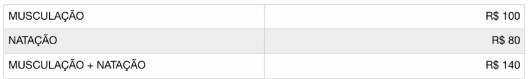
\includegraphics[width=0.7\linewidth]{images/exModalidades}
	\caption{Exemplo de modalidades}
	Fonte: pessoal.
	\label{fig:exModalidades}
\end{figure}

Para a execução deste sistema, no escopo inicial foi proposto três telas, porém no atual projeto contemplaremos apenas duas, sendo elas cadastro e consulta. Na tela de cadastro será possível realizar todos os cadastros do sistema da academia (Alunos, Modalidades e valores, vinculos Aluno x Modalidade/Pacote, etc), enquanto na tela de consulta podemos visualizar a situação das mensalidades dos alunos (Pendente/Vencidas/Pagas) e aplicar filtros de pesquisa.

Na tela de cadastro será informado, no módulo de aluno, informações mínimas como: documento, endereço, nome, modalidade/pacote etc. Já no módulo de modalidades faremos o cadastro dos tipos de modalidades oferecidas (a princípio apenas o nome) e seus respectivos valores, bem como os pacotes ofertados. Sendo assim, a construção das tabelas se dá conforme segue:

\begin{figure}[H]
	\centering
	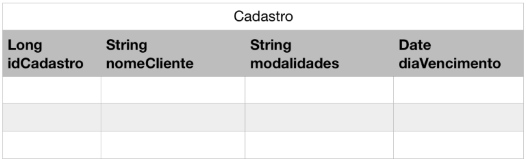
\includegraphics[width=0.7\linewidth]{images/tabelaCadastro}
	\caption{Tabela cadastro}
	Fonte: pessoal.
	\label{fig:tabelaCadastro}
\end{figure}

\begin{figure}[H]
	\centering
	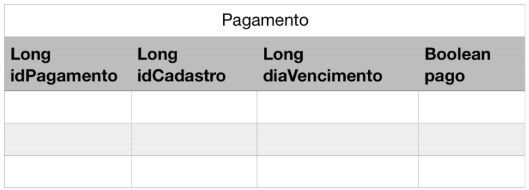
\includegraphics[width=0.7\linewidth]{images/tabelaPagamento}
	\caption{Tabela Pagamento}
	Fonte: pessoal.
	\label{fig:tabelaPagamento}
\end{figure}

Usaremos as tecnologias de Java e Swing (para o código e telas), MongoDB (para estruturar o banco de dados), Spring (para comunicação com o banco de dados) e GIT (para o gerenciamento de versão) para criar este sistema que pretende facilitar a consulta de pagamentos pendentes e controlar a matrícula dos alunos. Além disso, o atual escopo não prevê um controle financeiro (retorno de troco, quantidade recebida ou ainda fechamento de contas a pagar) e pode, futuramente, ser melhorado com a implementação destes itens ou ainda relatórios, controle de usuário etc.